\section{Methodology}
\label{methodology}

The proposed methodology consists of five sequential implementation phases 
that collectively support the development of a retrieval-augmented small 
language model system for medical AI applications \cite{yang2025rag, 
xiong2024rag}. These phases progress from corpus construction and model 
selection, through experimental evaluation and retrieval system 
implementation, to safety verification and clinical validation planning 
\cite{tam2024quest, labkoff2024aicds}.

\begin{figure*}[!t]
\centering
\includegraphics[width=0.75\textwidth,keepaspectratio]{Fig_Methodological_Implementation_Architecture.pdf}
\caption{Methodological Implementation Architecture}
\label{fig:methodology}
\end{figure*}

\subsection{Phase 1: Corpus Construction and Model Selection}
\label{phase1}

A domain-specific knowledge base was constructed by compiling 115 
authoritative medical documents: 112 PubMed articles covering major clinical 
domains \cite{krithara2023bioasq} and three clinical guidelines issued by the 
FDA, NICE, and NHS \cite{labkoff2024aicds}. \textbf{Scope and limitation:} 
the corpus comprises 115 documents and 556 semantic segments. This size 
supports focused evaluation and deployment in resource-constrained environments, but it does not represent the entirety of clinical medicine, 
and results should be interpreted within this defined scope. \textbf{
Coverage:} the corpus spans six clinical domains cardiology, endocrinology, neurology, oncology, immunology, and general medicine. \textbf{Scaling and 
updates:} future work will extend the corpus through periodic incorporation 
of updated clinical guidelines and integration of additional publicly 
available medical knowledge resources \cite{krithara2023bioasq}.

The documents were processed using a semantic chunking strategy that groups 
related content into logically coherent segments rather than relying on 
fixed-length partitioning \cite{pezoulas2023generative}, thereby preserving 
the contextual relationships among clinical concepts within each document. 
Text was extracted from PDF files and web pages and then normalized, after 
which natural language processing techniques were applied to segment the text 
into semantically coherent units. This process produced 556 segments of 512 
tokens each, with a 100-token overlap between adjacent segments to preserve 
contextual continuity; this overlap also enables cross-referencing of related 
clinical concepts by maintaining contextual associations between neighboring 
sections.

Each segment was embedded using the Sentence Transformers model \texttt{
all-MiniLM-L6-v2} from Hugging Face \cite{gu2020pubmedbert}. This model 
produces 384-dimensional semantic vectors and was selected for its 
computational efficiency and suitability for resource-constrained deployment; 
a comparative evaluation against biomedical-specific embedding models is 
planned for future work. Vector indexing was implemented using FAISS 
IndexFlatIP, with L2 normalization applied to vectors so that inner-product 
search corresponds to cosine similarity \cite{yang2025rag}, 
yielding an index size of less than 100\,MB. Overall, this corpus 
construction approach balances clinical coverage with computational efficiency 
to support deployment in environments with limited computational resources 
\cite{pezoulas2023generative, zamzmi2025smd}.

\subsubsection{Model Selection and Justification}

Two language models representing different positions on the efficiency--
quality spectrum were selected for evaluation: Gemma-2-2B-it  as the representative small language model (SLM), and 
Llama-2-7B-chat as the 
representative large language model (LLM).

\textbf{Justification for the small model (Gemma-2-2B-it).} Gemma-2-2B-it 
offers a favorable balance between parameter count and inference efficiency, 
making it suitable for deployment in resource-limited settings such as rural 
clinics or mobile diagnostic platforms \cite{xiong2024rag}. Prior studies 
indicate that retrieval-augmented smaller models can approach the performance 
of larger models on targeted question-answering tasks when supported by 
domain-specific knowledge sources \cite{yang2025rag, nishizaki2025reducing}. 
Gemma-2-2B-it requires approximately 4\,GB of memory and achieves 
sub-three-second latency, enabling deployment on modest hardware while 
remaining compatible with standard biomedical retrieval pipelines \cite{
zakka2023retrieval}. It therefore represents systems designed for 
efficiency-constrained healthcare environments.

\textbf{Justification for the large model (Llama-2-7B-chat).} Llama-2-7B-
chat was selected as the larger comparison model because it has been widely 
used in clinical and general natural language processing benchmarks \cite{
singhal2025toward}. Its 7B parameters and approximately 14\,GB memory 
requirement represent a computationally well-resourced configuration in which 
response completeness is prioritized over efficiency. The 
model has also been evaluated on medical question-answering tasks, supporting 
direct comparison with retrieval-augmented smaller models \cite{
amugongo2025retrieval}. Together, the comparison between Gemma-2-2B-it and 
Llama-2-7B-chat captures the trade-off between computational efficiency and 
response completeness in clinical AI systems.

\begin{figure*}[!t]
\centering
\includegraphics[width=\textwidth]{fig_rag_workflow_safety_routing.pdf}
\caption{RAG workflow, safety verification, and routing decision used in the proposed system.}
\label{fig:rag-workflow-safety-routing}
\end{figure*}

\begin{figure}[!t]
\centering
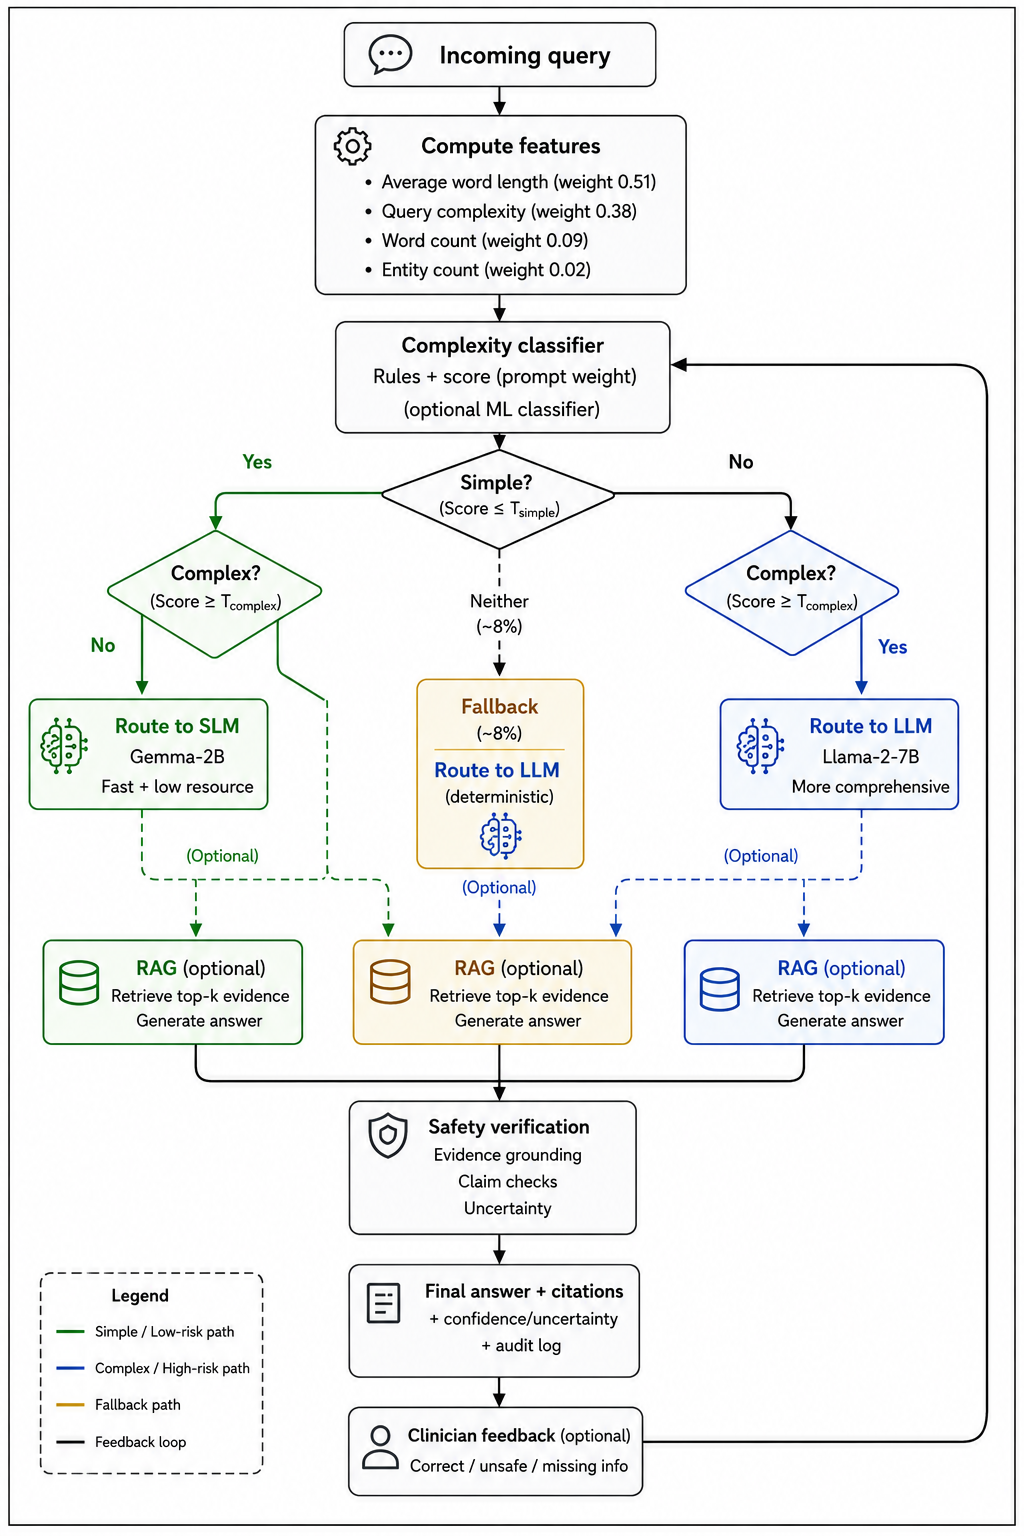
\includegraphics[width=\columnwidth]{fig_routing_decision.png}
\caption{Routing decision for assigning simple queries to the SLM and complex queries to the LLM, with optional retrieval augmentation and safety verification.}
\label{fig:routing-decision}
\end{figure}

\subsection{Phase 2: Experimental Framework and Evaluation}
\label{phase2}

A factorial $2\times2$ experimental design was used to evaluate the effect of 
retrieval augmentation across model configurations \cite{tam2024quest}. The 
core factorial analysis used three clinical queries: ``What is the treatment 
for diabetes and its associated management?'', ``How can AI assist in the 
diagnosis of disease?'', and ``What are the current guidelines for the 
management of hypertension?''. \textbf{Scope note:} this three-query set is 
an illustrative exemplar workload for demonstrating the token-F1 scoring 
protocol; it is not treated as a statistically powered quality benchmark. An extended evaluation set of 12 curated 
clinical questions spanning the six clinical domains which includes the 
three core queries was used for routing evaluation, load testing, and 
stability analysis. Each query was evaluated under two conditions: retrieval 
augmentation using the three most relevant chunks by cosine similarity, and a 
no-retrieval condition. Table~\ref{tab:query-mapping} in the Results section 
maps queries to their corresponding reported results.

The factorial design produced four experimental configurations SLM$\pm$RAG 
and LLM$\pm$RAG evaluated using the three core queries, for a total of 12 
experimental trials. This design separates model effects from retrieval 
effects and supports identification of suitable deployment configurations.

\subsubsection{Evaluation metrics and protocol}

The following evaluation measures were used. (1) \textbf{Response length 
(tokens):} an indicator of response size only, not a clinical quality metric. 
(2) \textbf{Latency:} inference time measured in seconds. (3) \textbf{RAG 
improvement (\%):} computed as $(N_{\mathrm{RAG}} - N_{\mathrm{NoRAG}}) / 
N_{\mathrm{NoRAG}} \times 100$ using token counts. (4) \textbf{Answer quality 
(F1):} the primary quality metric, computed as the harmonic mean of precision 
and recall based on token-level overlap between generated responses and 
reference answers. Reference answers were constructed for the evaluation 
dataset, and the scoring protocol is included in the reproducibility package. 
This approach follows common practice in generative question answering, where 
exact-match metrics are overly restrictive \cite{tam2024quest}. Statistical 
comparisons reported in this paper are based on F1 scores, while token-count 
improvements are reported separately as indicators of response length.

Model inference was implemented with FP16 precision, the \texttt{torch.no\_
grad()} execution context, key--value caching for token generation, and 
greedy decoding to minimize computational overhead. The combined active memory 
requirement for both models was approximately 9\,GB. Inference parameters 
were configured with a maximum of 64--128 new tokens, a minimum output length 
of 20 tokens, Greedy decoding was used for deterministic output; temperature 
and top-p parameters were set but inactive under this decoding strategy of at 
least 0.9.

\subsection{Phase 3: Retrieval-Augmented Generation with Evidence Grounding}
\label{phase3}

Throughout the factorial evaluation in this phase, \textbf{SLM}and 
\textbf{LLM}; these identifiers are used consistently throughout retrieval and generation. Post-hoc clinical-quality and faithfulness scoring 
(Table~\ref{tab:answer-quality}, Figure~\ref{fig:llm-judge-scores}) uses Qwen2.5-7B-Instruct as a separate, locally executed Hugging 
Face judge model; this judge operates independently of both the SLM and LLM 
inference pipelines and is applied only after response generation is complete.

\subsubsection{Query Routing}

Query routing is implemented as a \textbf{rule-based heuristic} , not a learned classifier. The routing logic assigns each 
incoming query to either the SLM or the LLM based on a set of deterministic 
criteria: queries are classified as \emph{simple} when they request a single 
clinical fact, definition, or direct guideline reference, and as \emph{
complex} when they involve multi-step reasoning, differential diagnosis, 
treatment comparison, or requests for synthesized evidence across multiple 
domains. Queries classified as complex are additionally flagged for retrieval 
augmentation prior to generation.

To verify implementation consistency, the heuristic was applied to a 240-query definition set (Appendix~\ref{app:routing-consistency}); held-out routing evaluation is planned for Phase~5 (Section~\ref{phase5}). Routing behavior on the Q1--Q12 workload is reported in Section~\ref{sec:routing-discussion}.

\subsubsection{Hybrid Retrieval Architecture}

This phase implements a hybrid retrieval architecture designed to improve 
response reliability through complementary retrieval mechanisms \cite{
yang2025rag, xu2025mega}. Dense retrieval captures semantic similarity 
between queries and knowledge base content using the sentence-
transformers/all-MiniLM-L6-v2 embedding model, which produces 384-
dimensional vectors indexed with FAISS IndexFlatIP. L2 normalization is 
applied to all vectors so that inner-product similarity is equivalent to 
cosine similarity, yielding an index of 556 vectors corresponding to the 
corpus segments described in Phase~1. Sparse retrieval complements the dense 
component by identifying exact clinical terminology and coding references that 
may not be well-represented in the embedding space. Results from both 
retrieval pathways are merged and re-ranked by a relevance scoring model that 
selects the top ten to fifteen documents per query. For the factorial 
evaluation, the three highest-ranked segments by cosine similarity are 
selected for context augmentation.

Retrieval latency was measured between 50 and 100\,ms per query under the 
experimental hardware configuration. This range supports near-real-time 
augmentation and is consistent with the sub-three-second end-to-end latency 
target established for the SLM deployment configuration (Section~\ref{phase1}). The hybrid strategy grounds generated responses in evidence 
retrieved from the biomedical corpus rather than relying solely on the 
parametric knowledge encoded in the language model weights, thereby reducing 
the exposure of generated outputs to factual drift or domain mismatch.

\subsubsection{Evidence Grounding and Prompt Construction}

Retrieved segments are injected into a structured prompt template prior to 
generation. The template positions the retrieved evidence before the query, 
instructing the model to confine its response to the provided context and to 
explicitly signal uncertainty when the retrieved material does not contain 
sufficient information to support a claim. This prompt structure enforces a 
soft grounding constraint at inference time and complements the claim-level 
verification mechanism applied in Phase~4 (Section~\ref{phase4}). Source 
segment identifiers are retained throughout the generation pipeline to support 
audit logging and traceability requirements described in Phase~5 
(Section~\ref{phase5}).

\subsection{Phase 4: Safety Verification and Hallucination Prevention}
\label{phase4}

A multi-stage verification process was implemented to improve the reliability 
of generated clinical responses \cite{asgari2022hallucination, 
nishizaki2025reducing}. The verification system includes an automated 
reviewer that analyzes each generated response and compares individual claims 
against the retrieved evidence, classifying each statement as supported, 
contradicted, or unsupported.

An audit logging mechanism records instances in which hallucinated statements 
are detected and blocked. These logs provide traceability for system outputs 
and support future improvements in model behavior, as well as compliance with 
regulatory and clinical validation requirements.

The safety framework operates through three verification levels aligned with 
clinical decision-support practice. The first level verifies the authenticity 
and provenance of retrieved evidence. The second level evaluates clinical 
plausibility by checking whether generated claims are consistent with the 
retrieved evidence and established medical reasoning. The third level performs 
confidence calibration, signaling uncertainty when the available evidence is 
insufficient to support a claim. As noted above, the system classifies each 
claim as supported, contradicted, or unsupported relative to the retrieved 
evidence, and claims classified as contradicted or unsupported are blocked or 
flagged before presentation to the user. Automated faithfulness scoring 
(Table~\ref{tab:answer-quality}) reports evidence-alignment rates for the RAG 
configurations; NoRAG comparability requires the extended faithfulness pass 
(\texttt{rag\_only=False}). The Phase~4 claim verifier is implemented as a 
design component, but end-to-end before/after blocking rates have not yet 
been quantitatively evaluated; these benchmarks will be reported together 
with the Phase~5 clinical validation results.

\subsection{Phase 5: Clinical Validation and Regulatory Compliance}
\label{phase5}

\textbf{Status:} Phase~5 is planned and has not yet been completed. The 
following describes the intended workflow for clinical validation and 
regulatory readiness.

This final phase is designed to evaluate the system within a clinical 
validation framework aligned with medical governance requirements \cite{
labkoff2024aicds}. A four-component evaluation framework similar to QUEST-
style assessment \cite{tam2024quest} is planned, in which licensed clinicians 
will evaluate generated responses for accuracy, clarity, and safety. Inter-
rater reliability will be measured, and the results will be documented in a 
comprehensive validation report.

\textbf{Concrete steps toward HIPAA, GDPR, and NHS-DTAC readiness} \cite{
jmir2024generative} include: (1) a Data Protection Impact Assessment (DPIA); 
(2) role-based access control mechanisms; (3) audit logging that records 
queries, retrieved segment identifiers, and system outputs without storing 
PHI; (4) PHI redaction or de-identification where applicable; (5) model risk 
management procedures, including validation and monitoring; and (6) refusal 
or uncertainty policies for unsupported or low-confidence claims. The current 
implementation already supports on-premise deployment, local processing, 
evidence-based claim verification, and audit logging; full regulatory 
validation and clinician-based evaluation will be conducted in the planned 
Phase~5 study.

\subsection{EIE Evaluation Framework}
\label{methodology:eie}

Operational resource use was assessed using the \textbf{EIE Framework} (Figure~\ref{fig:eie-framework}); measured outcomes are reported in Section~\ref{results:eie}. The framework reports NVML GPU energy and derived carbon emissions (Pillar~E), latency and VRAM observables under Context~A/B (Pillar~I), and reference electricity/hardware cost proxies (Pillar~Ec), each reported separately from clinical accuracy~\cite{ren2024reconciling, dauner2025ai, patterson2021carbon, strubell2019energy, epa2023egrid}.

\begin{figure}[!t]
\centering
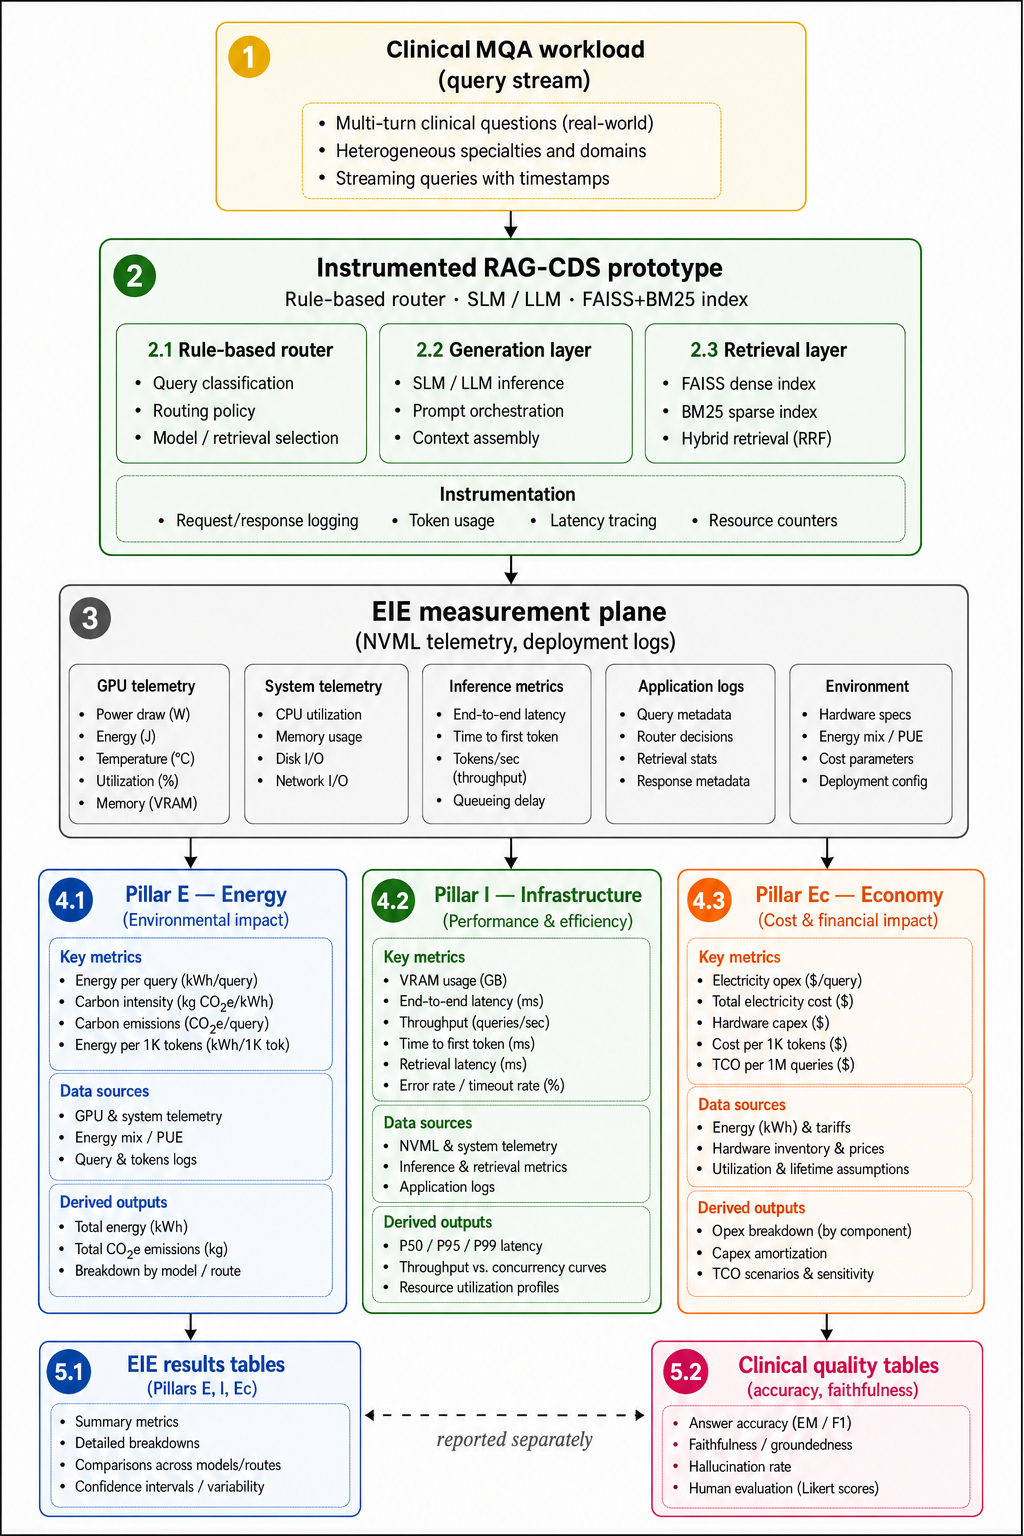
\includegraphics[width=\columnwidth]{fig_eie_framework_overview.png}
\caption{EIE framework overview for clinical MQA under RAG-CDS.}
\label{fig:eie-framework}
\end{figure}